% Set up the document class - this can be changed if a different format is required 
\documentclass[11pt,a4paper,oneside]{article}

% Include packages that contain additional features, for example including special mathematical characters and images in your document
\usepackage{amssymb,amsmath,graphicx}
\usepackage[T1]{fontenc} 
\usepackage[utf8]{inputenc}   % here are our umlauts...
\usepackage{graphicx} % ...and our graphics

\usepackage{bold-extra}
\usepackage[plainpages=false, pdfpagelabels, colorlinks=true, breaklinks=true, linkcolor=black, menucolor=black, urlcolor=black, citecolor=black]{hyperref}
\usepackage[font=sf, labelfont={sf,bf}, margin=1cm]{caption}
\usepackage[b]{esvect}
% Long equations
\usepackage{breqn} 
%include pdfs
\usepackage{pdfpages}
\usepackage{hyperref}
\usepackage{epstopdf}
%\usepackage{fullpage}
\usepackage{placeins}
\usepackage{subfig}

\usepackage{listings}
\lstloadlanguages{Python} % Load python syntax for listings, for a list of other languages supported see: ftp://ftp.tex.ac.uk/tex-archive/macros/latex/contrib/listings/listings.pdf
\DeclareFixedFont{\ttb}{T1}{txtt}{bx}{n}{9} % for bold
\DeclareFixedFont{\ttm}{T1}{txtt}{m}{n}{9}  % for normal
\usepackage{color}
\definecolor{deepblue}{rgb}{0,0,0.5}
\definecolor{deepred}{rgb}{0.6,0,0}
\definecolor{deepgreen}{rgb}{0,0.5,0}


% The beginning of the document...
\begin{document}
% configure standard code listings:
\lstset {
	language=Python,
	backgroundcolor=\color{white}, %%%%%%%
	basicstyle=\ttm,
	otherkeywords={self},            
	keywordstyle=\ttb\color{deepblue},
	emph={MyClass,__init__},          
	emphstyle=\ttb\color{deepred},    
	stringstyle=\color{deepgreen},
	commentstyle=\color{red},  %%%%%%%%
	frame=tb,                         
	showstringspaces=false,
	numbers=left
}

\renewcommand\thesubsection{\alph{subsection})}

% Please change the following accordingly...
\centerline{\LARGE \textbf{Artificial Intelligence - Exercise Sheet 10}}\vspace{0.5em}
\centerline{\large by Lucas-Raphael Müller}\vspace{2em}


\section{Image Compression using k-Means clustering}
\begin{figure}[ht]
   \centering
      %\subfloat[CAPTION]{BILDERCODE}\qquad
      \subfloat[]{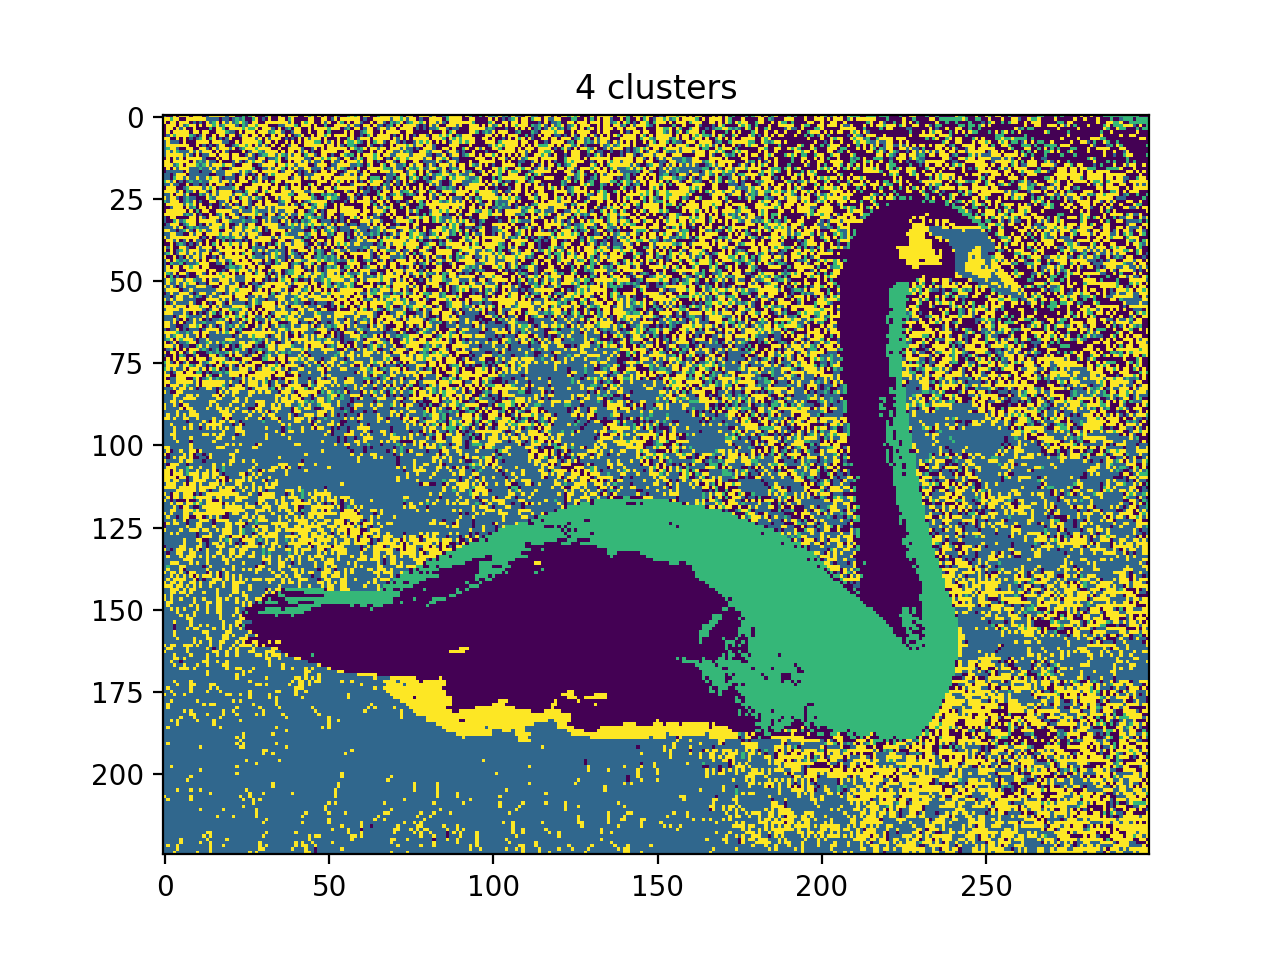
\includegraphics[width=0.45\textwidth]{figures/Figure_1.png}}\qquad
      \subfloat[]{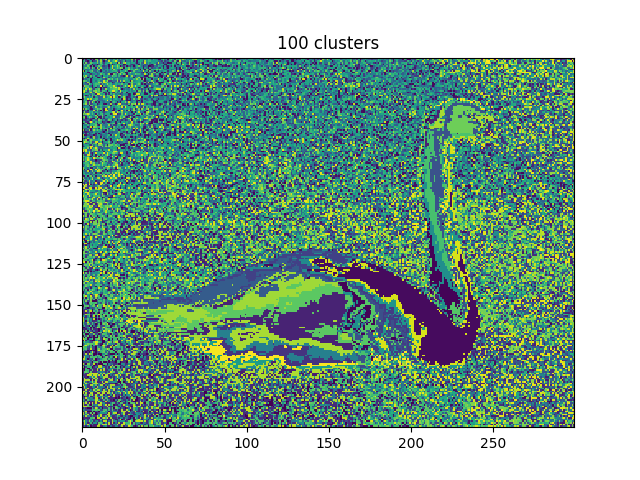
\includegraphics[width=0.45\textwidth]{figures/Figure_2.png}}\qquad
      \subfloat[]{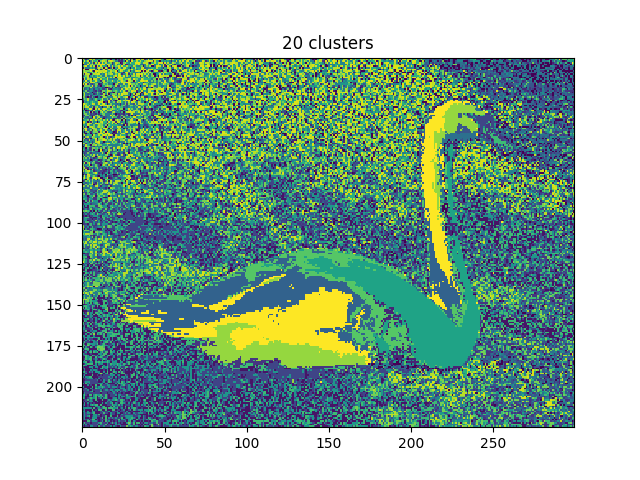
\includegraphics[width=0.45\textwidth]{figures/Figure_3.png}}
      \subfloat[]{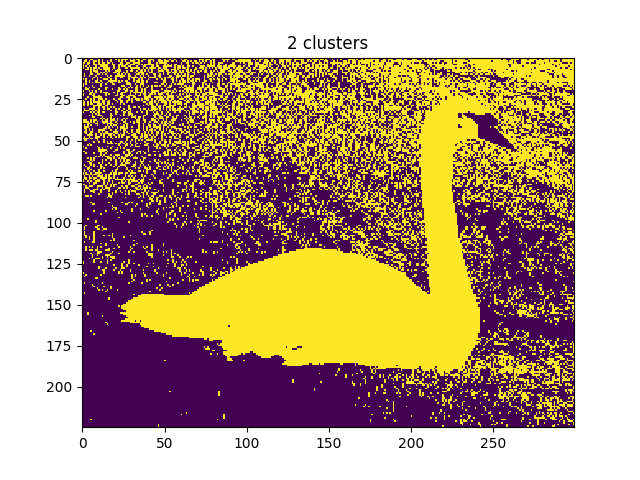
\includegraphics[width=0.45\textwidth]{figures/Figure_4.png}}
   \caption{Different numbers of clusters (centroids) in color space. Visualisation in original image space, computation in colour space.}
\end{figure}

\FloatBarrier

\section{Variational Autoencoder}
\lstinputlisting[language=Python]{source/vae.py}
\lstinputlisting[language=Python]{source/run_vae.py}
Couldn't completely finish. But did the implementation and it's working and produces state dicts.

\newpage
\section{Appendix: Python Source Code}
\label{sec:app}

\subsection{k-Means}
\lstinputlisting[language=Python]{source/k_means.py}


\end{document}
